\documentclass[a4paper,12pt]{article}

%%%%%%%%%%%%%%%%%%%%%%%%%%%%%%%%%%%%%%%%%%%%%%%%
% Packages
%%%%%%%%%%%%%%%%%%%%%%%%%%%%%%%%%%%%%%%%%%%%%%%%

\usepackage[right=2.5cm, left=2.5cm, top=2.5cm, bottom=2.5cm]{geometry} 
\usepackage[portuguese]{babel}
\usepackage[T1]{fontenc}
\usepackage[utf8]{inputenc}
\usepackage{enumerate}

% no indentation
%\usepackage{setspace}
%\setlength{\parindent}{0in}

\usepackage{graphicx} 
\usepackage{float}
\usepackage{xcolor}
\usepackage{tikz}
\usetikzlibrary{positioning}


\usepackage{mathtools}
\usepackage{amssymb, amsthm}

% headers
\usepackage{fancyhdr}
\usepackage{xurl}
\usepackage{hyperref}

%%%%%%%%%%%%%%%%%%%%%%%%%%%%%%%%%%%%%%%%%%%%%%%%
% Proper definitions
%%%%%%%%%%%%%%%%%%%%%%%%%%%%%%%%%%%%%%%%%%%%%%%%
\newcommand{\R}{\mathbb{R}}
\newcommand{\Q}{\mathbb{Q}}
\newcommand{\Z}{\mathbb{Z}}
\newcommand{\tr}{\operatorname{tr}}
\newcommand\eq{\mathrel{\overset{\makebox[0pt]{\mbox{\normalfont\tiny\sffamily def}}}{=}}}

\newtheoremstyle{exer}{}{}{\color{blue}}{}{\color{blue}\bfseries}{}{ }{}

\newtheorem*{aff}{Afirmação}

\theoremstyle{exer}
\newtheorem{exercise}{Exercício}

\theoremstyle{definition}

\newcommand{\enu}[1]{\textcolor{blue}{#1}}

%%%%%%%%%%%%%%%%%%%%%%%%%%%%%%%%%%%%%%%%%%%%%%%%
% Header (and Footer)
%%%%%%%%%%%%%%%%%%%%%%%%%%%%%%%%%%%%%%%%%%%%%%%%

\pagestyle{fancy} 
\fancyhf{}

\lhead{\footnotesize ANC: Lista 1}
\rhead{\footnotesize Prof. Hugo} 
\cfoot{\footnotesize \thepage} 


\begin{document}

%%%%%%%%%%%%%%%%%%%%%%%%%%%%%%%%%%%%%%%%%%%%%%%%
% Title section of the document
%%%%%%%%%%%%%%%%%%%%%%%%%%%%%%%%%%%%%%%%%%%%%%%%

\thispagestyle{empty} 

\begin{tabular*}{0.95\textwidth}{l @{\extracolsep{\fill}} r} 
    {\large \bf Introdução à Análise Numérica 2021.2} &  \\
    Escola de Matemática Aplicada, Fundação Getulio Vargas &  \\
    Professor Hugo A. de la Cruz Cancino &  \\ 
    Monitor Lucas Machado Moschen & Entrega 20/08/2021\\
    \hline \\
\end{tabular*} 
\vspace*{0.3cm} 

\begin{center}
	{\Large \bf Lista 1} 
	\vspace{2mm}
	%{\bf Lucas Machado Moschen}	
\end{center}  
\vspace{0.4cm}

\begin{exercise}
    Determine a representação em ponto flutuante (considerando precisão dupla)
    do número $x = 20.1$. 
\end{exercise}

\begin{enumerate}[{\color{blue} 1.}]
    \item \enu{Qual o número de máquina de 64 bits usado para armazenar
    $fl(x)$ no computador? }

    Uma sequência de passos que pode ser considerada é a seguinte: 

    \begin{enumerate}[(i)]
        \item Primeiro separamos a parte inteira da fracionária e
        transformamos
        ambas em binário: $20 = (10100)_2$ e $0.1 = (0\overline{0011})_2$. Para
        fazer essa conversão, na parte inteira basta dividir consecutivamente
        por 2 e agrupar os restos, enquanto a fracionária, basta multiplicar o
        número por 2 consecutivamente e tomar a parte inteira dos produtos.

        Assim, temos que $(20.1)_{10} = (10100.0\overline{0011})_2$. 

        \item Escrevemos o número em "notação científica", isto é, deixando
        apenas um 1 antes da vírgula, 
        $$
        (10100.0\overline{0011})_2 = 1.01000\overline{0011} \cdot 2^4
        $$

        \item Nesse caso, temos que o sinal é positivo e o expoente é 4.
        Adicionamos o viés de 1023 e obtemos que o expoente com viés será $1027
        = 2^{10} + 2^2 + 2^0 = (10000000011)_2$. 
        
        \item Agora basta verificar o último dígito da mantissa. Como 0.1 na
        base binária tem representação infinita, vamos precisar cortar. Temos
        5 dígitos antes da repetição 0011. Como temos 52 espaços, faltam 47
        para preencher e, então, teremos 11 vezes repetindo 0011 e, na últimas
        três vagas, 001. Como depois disso temos um 1, teremos que adicionar 1
        a mantissa, ficando com 010 na últimas posições. 
    \end{enumerate}
 
    Logo $[fl(20.1)]_{IEE754} = 0|100~000~000~11|01000~0011~\dots~0011~010$. 

    \item \enu{Determine o valor exato do erro arredondado. Ou seja,
    determine: $20.1 - fl(20.1)$}

    \begin{equation}
        \begin{split}
            fl(20.1) - 20.1 &= 1.010000011\dots 0011010 \cdot 2^4 - 1.010000011\dots 0011 0011 \dots \cdot 2^4 \\
            &=1010000011\dots0011010\cdot 2^{-48} - 1010000011\dots 0011001.1\overline{0011}\cdot 2^{-48} \\
            &= 10\cdot 2^{-48} - 1.1\overline{0011}\cdot 2^{-48} \\
            &= 2\cdot 2^{-48} - (1 + 0.5 + 0.1)\cdot 2^{-48} \\ 
            &= 0.4\cdot 2^{-48} = 0.1\cdot 2^{-46}.
        \end{split}
    \end{equation}

\end{enumerate}

\begin{exercise}
    Determine o equivalente decimal dos seguintes números de máquina em ponto
    flutuante.
\end{exercise}

Nesses exercícios, a solução é do tipo, 
$$
(-1)^s 2^{[c]_{10} - 1023} \cdot (1 + [m]_{10}), 
$$
em que $s$, $c$ e $m$ são os retângulos, respectivamente, com exceção dos subnormais. Claro que temos que
converter os números em decimal. Um arquivo python resolve esses problemas a
seguir no
Github\footnote{\url{https://github.com/lucasmoschen/ta-sessions/tree/master/Numerical_Analysis/lists/list1}}.
As soluções são, respectivamente, 
$$-3224, 1.32421875, 2.885642660251527e^{-308}, \operatorname{-Inf} \text{ e } \operatorname{NaN}.$$

\begin{enumerate}[{\color{blue} 1.}]
    \item \enu{\begin{tabular}{|c|c|c|}
            \hline
            1 & 10000001010
            &1001001100000000000000000000000000000000000000000000
            \\\hline
        \end{tabular}}

    \item \enu{\begin{tabular}{|c|c|c|}
            \hline
            0 & 01111111111
            & 0101001100000000000000000000000000000000000000000000
            \\\hline
        \end{tabular}}

    \item \enu{\begin{tabular}{|c|c|c|}
        \hline
        0 & 00000000000
        & 0101001100000000000000000000000000000000000000000000
        \\\hline
    \end{tabular}}

    \item \enu{\begin{tabular}{|c|c|c|}
        \hline
        1 & 11111111111
        & 0000000000000000000000000000000000000000000000000000
        \\\hline
    \end{tabular}}

    \item \enu{\begin{tabular}{|c|c|c|}
        \hline
        1 & 11111111111
        & 0000000000000000000000000000000000000000000000001111
        \\\hline
    \end{tabular}}

    \item \enu{Determine os próximos números de máquina para os números fornecidos
    nos itens anteriores, e escreva os mesmos na forma decimal.}

    A ideia nesse exercício é adicionar +1 no último termo. Em particular, os
    últimos dos itens são NaN. No primeiro e segundo item, adicionamos
    $2^{[c]_{10} - 1023 - 52}$. No terceiro item, adicionamos $2^{x + 1 - 1023
    - 52}$ em que $x$ é o número de {\it leading zeros}.

\end{enumerate}

\begin{exercise}
    Converte em binário ou converte em decimal, segundo seja o caso, e
    determine $fl(x)$: 
\end{exercise}

O arquivo python mencionado também faz essas contas. 

\begin{enumerate}[{\color{blue} 1. }]
    \item \enu{$x = 1/4$} 
    
    O binário é $0.01$.

    $fl\left(\frac{1}{4}\right) =  0~01111111101~0000000000000000000000000000000000000000000000000000$.

    \item \enu{$x = 1/3$}
    
    O binário é $0.\overline{01}$.

    $fl\left(\frac{1}{3}\right) = 0~01111111101~ 0101010101010101010101010101010101010101010101010101$.

    \item \enu{$x = 2/3$}
    
    O binário é $1.\overline{01}$.

    $fl\left(\frac{2}{3}\right) = 0~01111111110~ 0101010101010101010101010101010101010101010101010101$.

    \item \enu{$x = 0.9$}
    
    O binário é $0.1\overline{1100}$.

    $fl(0.9) = 0~01111111110~1100110011001100110011001100110011001100110011001101$

    \item \enu{$x = 0.\overline{1000111}$}
    
    O decimal é $71/127$.

    $fl\left(\frac{71}{127}\right) =
    0~01111111110~001111000111100011110001111000111100011110001111001$

    \item \enu{$x = 0.101\overline{100011}$}
    
    O decimal é $125/252$.

    $f_l\left(\frac{125}{252}\right) = 0~01111111101~1111101111101111101111101111101111101111101111110000$

\end{enumerate}

\begin{exercise}
    Para quais $k\in\mathbb{N}$ o número $5 + 2^k$ é representado de forma
    exata no computador. 
\end{exercise}

Temos que $5 + 2^k = 2^k + 2^2 + 2^0 = 10\dots 0101$, que o $k+1$-th digito é
1. Assim, 
$$
[5 + 2^k]_{10} = [1.00\dots 0101]_2\cdot 2^k.
$$
O sinal desse número é 0 e o expoente será o valor binário de $k - 1023$. A
mantissa terá tamanho $k$ mais uma sequência de 0 para completar as 52 casas. Logo, queremos que $0 \le k \le 52$. 

\begin{exercise}
    Considere a equação recursiva 
    \begin{equation}
        \label{eq:iteration}
        x_{n+1} = \frac{22}{7}x_n - \frac{3}{7}x_{n-1}; \qquad x_0 = 1, \quad x_1 = \frac{1}{7}
    \end{equation}
\end{exercise}

\begin{enumerate}[{\color{blue} 1.}]
    \item \enu{Demonstre que a equação acima tem solução $x_n =
    \left(\frac{1}{7}\right)^n$.} 

    Defina $S_n = [x_{n+1}, x_n]$. Teremos que $S_0 = [1/7, 1]$. Também defina
    $$
    A = \begin{bmatrix}
        22/7 & -3/7 \\
        1 & 0
    \end{bmatrix}, 
    $$
    em que $S_{n+1} = AS_n$. Portanto, teremos que $S_n = A^nS_0$. Para isso,
    vamos diagonalizar a matriz $A$. Os autovalores de $A$ são soluções da
    equação característica: 
    $$
    7\lambda^2 - 22\lambda + 3 = 0, 
    $$
    cujas soluções são $\lambda_1 = 3$ e $\lambda_2 = 1/7$. Se $P$ é a matriz
    de autovetores, teremos que 
    $$
    S_n = P\begin{bmatrix}
        3^n & 0 \\ 0 & 7^{-n}
    \end{bmatrix}P^{-1}S_0, 
    $$
    isto é, $x_n = A3^n + B7^{-n}$, de forma que $x_0 = A + B$ e $x_1 = 3A +
    B/7$. Resolvendo o sistema de equações, obtemos que $A = 0$ e $B = 1$,
    isto é, 
    $$
    x_n = \left(\frac{1}{7}\right)^n.
    $$

    \item \enu{Implemente o processo iterativo \eqref{eq:iteration} para calcular
    $x_n$.}

    A implementação em Python se encontra no mesmo link no Github.     

    \item \enu{Compare para diferentes valores de $n$ os valores de $x_n$ obtidos
    usando a solução em a) e usando a implementação computacional feita em b).
    Por que a partir de um certo valor de $n$ os valores são completamente
    diferentes? Reflita sobre isso!}

    Considere a figure \ref{fig:fig1} para comparar os valores de $x$. Observe
    que usando a versão iterativa anda com a solução direta, mas a partir de
    um dado instante, expressão diverge para $-\infty$. Observamos que existe
    um dado momento em que a solução troca de sinal. Essa troca de sinal, faz
    com que as soluções subsequentes sejam sempre negativas e em diante elas
    continuem reduzindo, infinitamente.   

    \begin{figure}
        \centering
        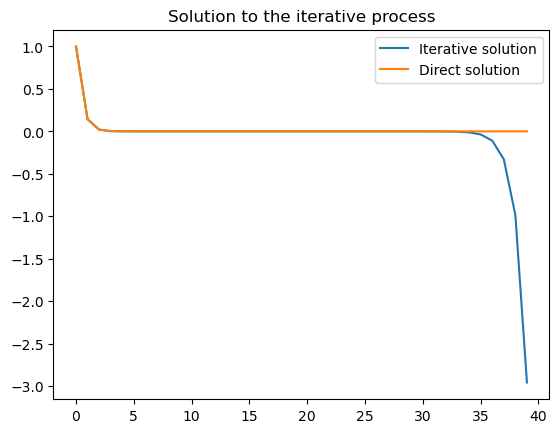
\includegraphics[width=0.7\textwidth]{image_exercise5.png}
        \caption{Comparação dos valores de x para a implementação computacional e usando a solução direta.}
        \label{fig:fig1}
    \end{figure}    

    \item \enu{Faça uma análise de estabilidade do algoritmo implementado em b)
    para calcular $x_n$.}

    Suponha que $x_1 = 1/7 + \delta$, em que $\delta$ é, em geral, um pequeno
    número. Nesse caso, temos que a solução será 
    $$
    x_n = \frac{7}{20}\delta\cdot 3^n + \left(1 + \frac{7}{20}\delta\right)\left(\frac{1}{7}\right)^n = \left(\frac{1}{7}\right)^n + \frac{7}{20}\delta(3^n + 7^{-n}).
    $$
    Nesse caso, se $\delta < 0$, a solução converge para $-\infty$ (que é o
    caso do exercício anterior) e, se $\delta > 0$, a solução converge para $+
    \infty$. 

\end{enumerate}

\end{document}